% CONSORT flow diagram for the eRegQual trial.
% Based on: https://texample.net/tikz/examples/consort-flowchart/
%
% Compile tfrom .tex to .png using:
% pdflatex eRegQual_CONSORT.tex
%
% Convert to a high-res PNG using:
% sips -s format png --resampleWidth 10000 eRegQual_CONSORT.pdf --out eRegQual_CONSORT.png

\documentclass{article}
\usepackage[latin1]{inputenc}
\usepackage{tikz}
\usetikzlibrary{shapes,arrows}
\usepackage{enumitem}

\newcommand*{\h}{\hspace{5pt}}% for indentation
\newcommand*{\hh}{\h\h}% double indentation

\begin{document}
\pagestyle{empty}
\pagecolor{white}
\begin{center}
  % setting the typeface to sans serif and the font size to small
  % the scope local to the environment
  \sffamily
  \footnotesize
  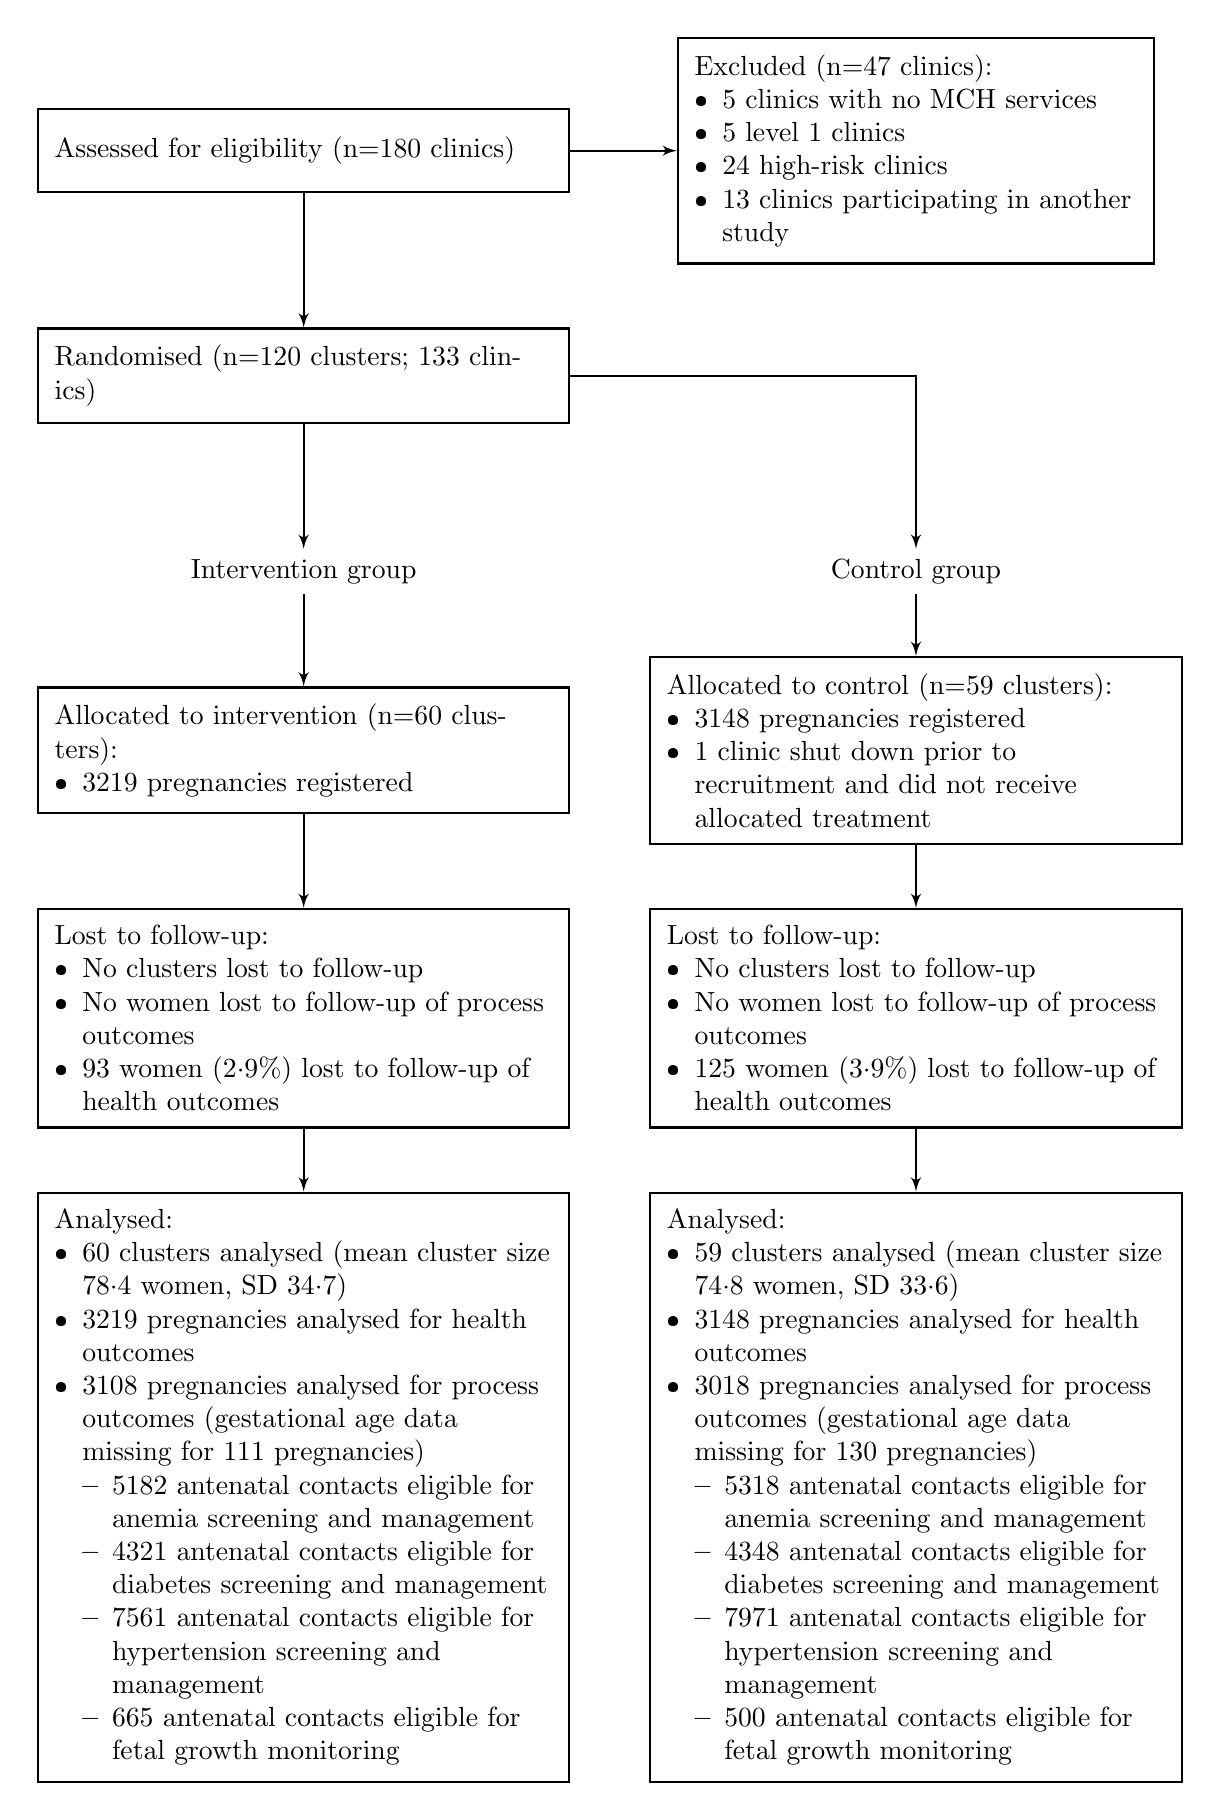
\begin{tikzpicture}[auto,
    block_center/.style ={rectangle, draw=black, thick, fill=white,
      text width=8em, text centered,
      minimum height=4em},
    block_left/.style ={rectangle, draw=black, thick, fill=white,
      text width=16em, text ragged, minimum height=4em, inner sep=6pt},
    block_noborder/.style ={rectangle, draw=none, thick, fill=none,
      text width=18em, text centered, minimum height=1em},
    block_assign/.style ={rectangle, draw=black, thick, fill=white,
      text width=18em, text ragged, minimum height=3em, inner sep=6pt},
    block_lost/.style ={rectangle, draw=black, thick, fill=white,
      text width=16em, text ragged, minimum height=3em, inner sep=6pt},
      line/.style ={draw, thick, -latex', shorten >=0pt}]
    % outlining the flowchart using the PGF/TikZ matrix function
    \matrix [column sep=10mm,row sep=8mm] {
      % Assessment
      \node [block_assign] (assessment) {Assessed for eligibility (n=180 clinics)};
      & \node [block_left] (excluded1) {Excluded (n=47 clinics): \\
          \begin{itemize}[leftmargin=*, nolistsep]
            \item 5 clinics with no MCH services
            \item 5 level 1 clinics
            \item 24 high-risk clinics
            \item 13 clinics participating in another study
          \end{itemize}}; \\
      % Randomised
      \node [block_assign] (randomised) {
          Randomised (n=120 clusters; 133 clinics)}; \\
      & \\
      % Groups
        \node [block_noborder] (i) {Intervention group}; 
      & \node [block_noborder] (c) {Control group}; \\
      % Allocation
        \node [block_assign] (i_T0) {Allocated to intervention (n=60 clusters): \\
          \begin{itemize}[leftmargin=*, nolistsep]
            \item 3219 pregnancies registered
          \end{itemize}}; 
      & \node [block_assign] (c_T0) {Allocated to control (n=59 clusters): \\
          \begin{itemize}[leftmargin=*, nolistsep]
            \item 3148 pregnancies registered 
            \item 1 clinic shut down prior to recruitment and did not receive allocated treatment
          \end{itemize}}; \\
      % Loss to follow-up
      \node [block_assign] (i_followup) {
        Lost to follow-up:
        \begin{itemize}[leftmargin=*, nolistsep]
          \item No clusters lost to follow-up
          \item No women lost to follow-up of process outcomes
          \item 93 women (2${\cdot}$9\%) lost to follow-up of health outcomes
        \end{itemize}};
	  & \node [block_assign] (c_followup) {
      Lost to follow-up:
      \begin{itemize}[leftmargin=*, nolistsep]
        \item No clusters lost to follow-up
        \item No women lost to follow-up of process outcomes
        \item 125 women (3${\cdot}$9\%) lost to follow-up of health outcomes
      \end{itemize}}; \\
      % Analysis
      \node [block_assign] (i_analy) {Analysed:
        \begin{itemize}[leftmargin=*, nolistsep]
          \item 60 clusters analysed (mean cluster size 78${\cdot}$4 women,
                SD 34${\cdot}$7)
          \item 3219 pregnancies analysed for health outcomes
          \item 3108 pregnancies analysed for process outcomes (gestational age
                data missing for 111 pregnancies)
          \begin{itemize}[leftmargin=*, nolistsep]
            \item 5182 antenatal contacts eligible for anemia screening and management
            \item 4321 antenatal contacts eligible for diabetes screening and management
            \item 7561 antenatal contacts eligible for hypertension screening and management
            \item 665 antenatal contacts eligible for fetal growth monitoring
          \end{itemize}
        \end{itemize}};
    & \node [block_assign] (c_analy) {Analysed:
        \begin{itemize}[leftmargin=*, nolistsep]
          \item 59 clusters analysed (mean cluster size 74${\cdot}$8 women,
                SD 33${\cdot}$6)
          \item 3148 pregnancies analysed for health outcomes
          \item 3018 pregnancies analysed for process outcomes (gestational age
                data missing for 130 pregnancies)
          \begin{itemize}[leftmargin=*, nolistsep]
            \item 5318 antenatal contacts eligible for anemia screening and management
            \item 4348 antenatal contacts eligible for diabetes screening and management
            \item 7971 antenatal contacts eligible for hypertension screening and management
            \item 500 antenatal contacts eligible for fetal growth monitoring
          \end{itemize}
        \end{itemize}};
      \\
    };% end matrix
    % connecting nodes with paths
    \begin{scope}[every path/.style=line]
      % paths for enrollemnt rows
      \path (assessment) -- (excluded1);
      \path (assessment) -- (randomised);
      \path (randomised) -- (i);
      \path (i)          -- (i_T0);
      \path (randomised) -| (c);
      \path (c)          -- (c_T0);
      \path (i_T0)       -- (i_followup);
      \path (c_T0)       -- (c_followup);
      \path (i_followup) -- (i_analy);
      \path (c_followup) -- (c_analy);
    \end{scope}
  \end{tikzpicture}
\end{center}
\end{document}